\section{Le POSIX 1003.1}
 
Traditionnellement les systèmes qui implémentaient la norme POSIX avaient un système simple et puissant de permissions mais qui cependant posait certains problèmes. En effet, les différentes versions d'ACL disponibles étaient incompatibles entre elles.
 
Pour normaliser les problème de sécurité sur les systèmes POSIX (ACL en faisant partie), un groupe a été formé pendant la définition de la famille de normes POSIX 1003.1. Les premiers documents POSIX qui ont pris en compte ces questions étaient les documents 1003.1e (\emph{System Application Programming Interface}) et 1003.2c (\emph{Shell and Utilities}), cependant, le premier draft était trop ambitieux. En effet, le groupe responsable pour la normalisation avait divisé ses efforts sur un grand nombre de domaines qui comportaient les \emph{Access Control Lists} (ACL), les \emph{Audit}, les \emph{Capability},les \emph{ Mandatory Access Control }(MAC), et l'\emph{Information Labeling}\cite{aclsuse}.
 
En Janvier de 1998\cite{aclsuse} le financement pour ce projet à été suspendu, par contre, le travail n'était pas prêt. De toute façon le dixsèptieme draft a quand même été rendu public\cite{posix17}.
 
Après cette publication, des systèmes UNIX appelés "\emph{trusted}" (Trusted Solaris, Trusted Irix, Trusted AIX) ont été développés à partir du draft 17. Ces systèmes ne sont pas complètement compatibles entre eux. Heureusement aujourd'hui la plupart des systèmes UNIX et UNIX-like supportent les ACL. Ces implémentations sont usuellement compatibles avec le draft 17. Le projet TrustedBSD implémente aussi les ACL sur les système BSD. Les ACL sont apparues sur les Macs en 2003 avec la RELEASE MAC FreeBSD.
 
Les ACL sont une évolution du système de permissions traditionnel présent dans pratiquement tous les systèmes UNIX, alors, avant d'expliquer les ACL on va d'abord parler du modèle traditionnel.
 
\subsection*{Système de permissions traditionnel}
 
%Les groups et les permissions
Le modèle traditionnel POSIX offre trois classes d'utilisateurs qui sont: le propriétaire (\emph{owner}), le groupe propriétaire (\emph{group}) et les autres utilisateurs (\emph{others}). Chaque groupe a un octet que indique les permissions de lecture (\emph{\textbf{r}ead}), d'écriture (\emph{\textbf{w}rite}) et d'exécution (\emph{e\textbf{x}ecute}).
 
%Explication simple
Après les trois octets peut venir le \emph{Set User Id}, \emph{Set Group Id} et le \emph{Sticky Bit} qui peuvent être utilisés dans certain cas. Il faut faire attention avec le \emph{Sticky Bit}, il permet aux utilisateurs normaux d'exécuter les utilitaires comme l'administrateur(\emph{root}), donc une faille de sécurité dans une application utilisant le \emph{Sticky Bit} peut compromettre le système entier.
 
%Le droit du root
Seul le \emph{root} peut créer les groupes et changer les associations de groupes. Il peut aussi changer les propriétaires.
 
\subsection*{Les ACL}
 
%Definitions de base
Chaque ACL est une ensemble de règles d'accès. Dans une modèle de sécurité utilisant les ACL, si une entité fait une requête pour accéder aux données, il faut consulter les la liste d'ACL pour savoir si nous avons la permission pour l'opération demandé. Les règles possibles peuvent être consultées dans le tableau ci-dessous(\ref{entree}).

\begin{center}
\begin{tabular}{|l|l|}
  \hline
    \multicolumn{2}{|c|}{Les types de ACL} \\
  \hline
\textbf{Type d'entrée} & \textbf{format} \\
  \hline
Propriétaire & user::rwx \\
Utilisateur nommée & user:name:rwx \\
Groupe propriétaire & group::rwx \\
Groupe nommée & group:name:rwx \\
Masque & mask::rwx \\
Autres & other::rwx \\
  \hline
\end{tabular}
\label{tab:entree}
\end{center}
 
Les règles sont formées par un indicateur de classe (comme les classes du système traditionnel), l'identificateur pour préciser de quel utilisateur ou groupe on parle puis les octets de permissions.

Les ACL équivalentes au mode simple de permissions s'appellent les ACL minimales. Une ACL minimale possède 3 entrée (propriétaire, groupe propriétaire et autres) qu'on peut convertir directement. Si les ACL possèdent des entrées supplémentaires, ont les appelle ACL étendues. Toutes les ACL étendues doivent avoir une entrée masque et peuvent contenir théoriquement autant d'entrées que l'on désire. Ce numéro d'entrée peut-être limitée pour chaque implémentation et qu'il est aussi important pour les performances.

Quelquefois on a des application qui ne sont pas programmer pour fonctionner avec les ACL, cela veut dire que l'on doit créer une relation pour convertir les ACL vers le système traditionnel, de façon que ces application ne donnerons pas de façon inattendue plusieurs droits aux utilisateurs ou groupes. 

Quand le programme utilise des ACL minimales ce problème n'arrive jamais: la relation entre ces ACL et le système traditionnel est directe. Par contre, dans les ACL étendues cela pose une problème. Les propriétaires et les autres seront directement associe avec les classes de même nom, par contre, les entrées de groupe et utilisateur nommé avec le groupe propriétaire seront tous associés avec la classe du groupe propriétaire. Par conséquent, le sens du classe groupe propriétaire doit être redéfinie comme la limite supérieure des permissions de chaque entrée dans pour la classe groupe.

Comme dans les ACL étendues on peut avoir des entrées avec plusieurs utilisateurs et/ou groupes nommés, quelques unes ces entrées peuvent contenir des permissions que la classe groupe n'aura pas, alors, on peut avoir des incohérences dans certain cas. 


Cette question peut se résoudre avec l'utilisation d'un masque. Comme on peut l'observer dans le figure (\ref{fig:img_acl-mapping}), il y a deux cas:  Les ACL minimales où la classe groupe est référencée pour l'entrée du groupe propriétaire. Les ACL étendues de la classe groupe seront trouvées en faisant un masque avec les permissions du groupe propriétaire, les permissions des utilisateurs nommés et groupe nommés. Cela rend difficil le calcul de classe groupe. 

\begin{figure}[htbp]
\centering
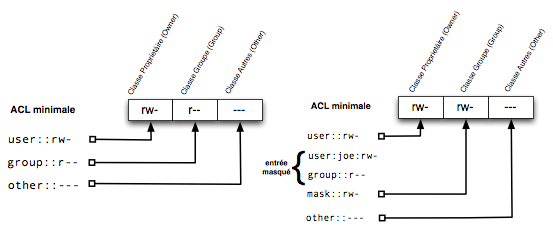
\includegraphics[height=3in]{img/acl-mapping.jpg}
\caption{caption}
\label{fig:img_acl-mapping}
\end{figure}
 
 
Pour assurer le cohérence, quand une application change les permissions (par exemple le commande \emph{chmod}) les ACL sont modifiées de façon a reproduire cette modification.
 
On a dit que les permissions du masque sont calculées comme la limite supérieure de tous les entrées dans le classe groupe. Avec les ACLs étendus, on a besoin de masquer les permissions. Comme l'exemple du tableau (\ref{tab:masquee}), les permission des entrées de la classe groupe et qui aussi sont présentes dans le masque sont appliquées. Si une permission est absente dans le masque, c'est à dire qu'aucune entrée de groupe ne peut avoir cette permission, on dit dans ce cas que l'entrée est masquée.
 
\begin{center}
\begin{tabular}{|l|l|l|}
  \hline
    \multicolumn{3}{|c|}{La masque de permissionL} \\
  \hline
\textbf{Type} & \textbf{Format} & \textbf{Permission} \\
  \hline
Utilisateur nommée & user:jean:r-x & r-x\\
  \hline
Masque & mask::rw- & rw-\\
  \hline
\multicolumn{2}{|c|}{Permission Effective} & rw-\\
  \hline
\end{tabular}
\label{tab:masque}
\end{center}


Par être consistent, dans une application que utilise les ACL étendu, le permission du groupe propriétaire est toujours calculée comme la union entre le permission de ce groupe e la masque.  
 
\subsection*{Algorithme de vérification}
 
Pour vérifier les droits d'accès d'une objet du système de fichier, il y a une algorithme assez simple.
 
%changer le titre et la langue
\begin{algorithm}
\caption{Vérifie se une utilisateur peut ou ne peut pas accéder une objet du système de fichier}
\label{algacl}
\begin{algorithmic}
\IF{l'identifiant de l'utilisateur du processus est le propriétaire}
\STATE l'entrée du propriétaire détermine l'accès
\ELSIF{l'identifiant d'utilisateur du processus correspond à une entrée d'utilisateur nommé dans la table des ACL}
\STATE l'entrée détermine l'accès
\ELSIF{un des identifiants de groupe du processus correspond au groupe propriétaire et l'entrée contient les permissions requises}
\STATE l'entrée détermine l'accès
\ELSIF{
un des identifiants de groupes correspond à un des groupe nommés et cette entrée contient les permissions requises}
\STATE l'entrée détermine l'accès
 
\ELSIF{
Un des identifiants de groupe du processus correspond au groupe propriétaire ou correspond à un des groupes nommés mais ni le groupe propriétaire ni aucun des groupes nommé contient les permission requises.}
\STATE ceci détermine que l'accès est interdit
 
\ELSE
\STATE l'entrée autre détermine l'accès
\ENDIF
 
%
\IF{
l'entrée qui détermine l'accès est l'entre du propriétaire ou l'entrée autres qui contient les permissions requises}
\STATE 
l'accès est autorisé
\ELSIF{l'entrée correspondante est l'utilisateur nom, ou le groupe propriétaire ou le groupe nommé et cette entrée contient les permissions requises et l'entrée masque contient aussi les permission. (ou il n'y a pas d'entrée masque)
}
\STATE l'accès est autorisé
 
\ELSE
\STATE l'accès n'est pas autorisé
\ENDIF
\end{algorithmic}
\end{algorithm}
 
 
\subsection*{Héritage mécanisme}
\label{sec:heritage}
 
Le système POSIX règle non seulement les droits d'accès aux objets du système de fichiers, mais aussi le mécanisme d'Héritage. Les ACL sont partagés en deux types, les 
ACL d'accès (qu'on a vu jusqu'à maintenant) et les ACL par défaut qui comprennent les règles d'héritage.
 
Quand on parle de l'héritage, on parle des droits qui sont attribués aux objets du systèmes de fichiers au moment où ils sont crées. Il y a un seul type d'objet qui peut être associe avec les ACL par défaut les répertoires. Il faut dire que il n'y a pas de sens pour les ACL par défaut pour les fichiers car on ne peut pas créer un fichier à l'intérieur d'un fichier. Aussi les ACL par défaut et les 
ACL d'accès sont complètement indépendant.
 
Si un répertoire est crée dans une autre, si le première répertoire a ACL par défaut, avec le mécanisme d'héritage, le deuxième aura le même ACL que le premier (défaut  et accès). Les objets qui ne sont pas des répertoires, devons hériter les ACL par défaut seulement.
 
Chaque \emph{system call} qui crée les objets du système de fichier a un \emph{mode parameter}. Ce paramètre peut contenir neuf octets de permission pour chaque classe (propriétaire, groupe et les autres). Les permissions de chaque objet créée sont l'intersection des permissions définies pour les ACL par défaut et le \emph{mode parameter}.
 
Le système traditionnel a une commande pour désigner les modes de permissions par défaut pour les nouveaux fichiers et répertoires: le commande \emph{umask}. Quand il n'y a aucune ACL par défaut, la permission effective est déterminé par le \emph{mode parameter} moins les permissions configurés avec \emph{umask}.
 